\chapter{Basics}

\section{Optimization in Deep Learning}
Optimization is a core part of deep learning, as it is the
foundation of the learning process. However, optimization in the context of deep
learning differs from traditional optimization in several ways. This section
focuses on these differences and further challenges of optimization in
deep neural networks. Most of the sections are inspired by
\cite{Goodfellow-et-al-2016}.

\subsection{Difference to traditional optimization}\label{sub:1} 
With traditional optimization, we optimize directly on the data that we want to
perform later. However, in deep learning, we usually do not have access to the
test data. Consider autonomous driving. Here, the data the self-driving agent
has to act on will be generated while driving, with no chance of getting it in
advance. But we can capture data of other cars and optimize on them indirectly.
The hope beeing, that the distribution of the training set is similar to the one
of the later test set, so that reduction of training error will result in recution
test error.

Formally, we want to reduce the test error given by
\begin{align}\label{eq:1}
    J(\theta) = E_{(x,y)\sim p_{data}} L(f(x;\theta), y)
\end{align}
where $L$ is the Loss-Function, $f(x;\theta)$ the output of the model with
respect to the input $x$, parameters $\theta$ and labels $y$ for the
input. This equation is known as \textbf{risk}. However, during the training
process, we only have access to the training set which is distibuted according
to the empirical distribution $\hat{p}_{data}$ rather than true underlying
distribution $p_{data}$. Therefore, we can only optimize the funtion
\begin{align}
    J(\theta) = E_{(x,y)\sim \hat{p}_{data}} L(f(x;\theta), y)
\end{align}
which is known as \textbf{empirical risk}.

To overcome this issue and convert the problem back to a normal optimization
problem, we use a technique called \textbf{empirical risk minimization}. Here,
the expectation over the empirical distribution is approximated by the arithmethic
mean.
\begin{align}\label{eq:3}
    J(\theta) = E_{(x,y)\sim \hat{p}_{data}} L(f(x;\theta), y) = \frac{1}{m} \sum_{i=1}^m L(f(x^{(i)}; \theta), y^{(i)})
\end{align}
As the training set is restricted in size, this approach quickly leads to
overfitting, where the network memorizes the training set. Althought the
performance on the training set still improves, the performance on the test set
worsens again. Reguralization strategies try to decrease this difference between
the datasets. Section \ref{sub:Generalization} describes the problem and some
solutions in more detail.


\subsection{Minibatch Algorithms}\label{sub:Minibatch}
We have seen in equation \ref{eq:3} that we use the mean over the whole training
set to compute the empirical risk. From a computational perspective, this is
rather expensive. That is why we normally only use a subset of the training set
for each parameter update. These subsets are called \textbf{batches}. Some statistical
considerations justify this.

The standard error of the mean is given by $\frac{\sigma}{\sqrt{n}}$, where $n$
is the number of training examples. The root in the denominator $\sqrt{n}$ means
that increasing the number of training examples to estimate the gradient will
only lead to a sublinear decrease of the standard error. On the other hand,
computation time scales linear with the number of training examples. A training
set 10 times larger requires ten times more computation time, but reduces the
standard error only by $\sqrt{10}$. Therefore, large batches are often
unattractable. The second factor is redundancy in the training set. As the
training examples are drawn from the same underlying distribution, the mean of a
subset will not differ much from the whole training data, but requires much less
computation time.

Most loss-functions allow us to divide the data into batches easily. The most
common example for classification is maximum likelyhood, which is defined as:

\begin{align}
    \theta_{ML}
    & = argmax_{\theta} p_{model}(X; \theta) \\
    & = argmax_{\theta} \prod_{i=1}^m p_{model}(x^{(i)}; \theta)
\end{align}

If we convert it to log-space, the product decomposes into a sum:

\begin{align}
    \theta_{ML} = argmax_{\theta} \sum_{i=1}^m log p_{model}(x^{(i)}; \theta)
\end{align}

In this space, we can easily divide the sum into batches and train on them
seperatly. The same idea can be applied to the gradient:
\begin{align}
    \nabla_\theta J(\theta)=E_{x,y\sim \hat{p}_{data}} \nabla_\theta log(p_{model}(x,y;\theta))
\end{align}

Optimization algorithms which use the whole training set are called
\textbf{batch} or \textbf{deterministic} algorithms, while deterministic is
prefered, as the term batch is also used in minibatch methods. The other extreme
are \textbf{stochastic} or \textbf{online} methods, where only one training
example is processed at a time. In between lie the methods, where more than one
training example is used, but not all. These are called \textbf{minibatch}
methods and are most commonly used in machine learning. A typical example for
stochastic methods is stochastic gradient descent, see section \ref{SGD}.


Both methods have their advantages beyond the computational perspective. While
large batches offer a more accurate estimate of the gradient, small batches can
add a regularization effect. They add some noise to the gradient, and seem to
lead the optimization algorithm to stable or wide minima. These are minima,
where regardless of the starting position in a certain range around the minima,
an optimization algorithm will still go back to that minima. The higher the
range, the wider the minima is. The current state of reseach suggests that wider
minima have better generalization capabilities. This idea is supported by the
work of Keskar et al. \cite{keskar2016large}, who argued that larger batches
converge to sharp minimas, whereas small converge to flat.

To get an less biased esimate of the gradient, it is important to sample the
mini-batches randomly. This can be achieved by sampling the minibatches
uniformly out of the training data. However, that would lead to a large
computational effort every time we want to construct a batch. Fortunally, it
seems sufficient to shuffle and divide the training data into batches only once.

Another property is that the gradient of minibatch algorithms like stochastic
gradient descent give an unbiases estimate of the gradient, as long as the
training data is only used once. In this case, the data is drawn from the real
distribution $p_{data}$. But as soon as examples are reused, the training data
distribution gets biased. However, because the size of training examples is limited,
multiple passes through the training data are useful.

\subsection{Challenges in Optimization of Neural Networks}
In the last part, we demonstrated how optimization in deep learning differs from
traditional optimization from a statistical point of view. This difference is
emphasized further by other factors, in particular the loss landscape. While in
traditional machine learning, the loss landscape was convex, for deep neural
networks, it is highly non-convex. This part will summarize some of these
problems and their implications for deep learning.


\subsubsection{Local Minima}\label{sub:Local_minima}
In convex optimization problems, every local minima is guaranteed to be the
global minimum. Therefore finding a minimum is a sufficient enough condition to
stop. In neural networks however, the loss landscape is highly non-convex. That
is the reason why there is no guarantee that a found minimum is the global one.
Proof that local minima exist can be constructed quite easily.

One example is the weight space symetrie. Suppose you swap out nodes i and j by
swapping their incoming and outgoing weights. Then the activation in the next
and all subsequent layers of the networks will stay the same, but the networks
are located at different places on the loss landscape, therefore creating two
local minima. Although a large number of these local minima exist, they form no
problem for optimization. As mentioned, the swap will lead to the same
activation, therefore the networks will performe the same on the data and the
value of these local minimas will be equal.

However, there can also exist local minima with high cost compared to the global
minimum. In theorie this was believed to be an issue, but in practice it seemed
to cause no problem. Recently, some theoretical work support these findings.
Chromanska et al. \cite{choromanska2015loss} applied spin glass theory from
physics to neural networks. This allowed them to verify that for large networks,
local extrema with higher cost are exponentially likely to be saddle points.
Therefore, all local minima are approximately of the same cost, which is close
to the global optimum and an optimization algorithm is unlikely to get stuck in
a local minimum with high cost.

\subsubsection{Saddle Points}\label{prob:3}
Saddle points are another type of local extrema where the gradient is 0. In
contrast to local maxima or minima where the Hessian only has negative or
positive eigenvalues, the Hessian of saddle points has both positive and
negative eigenvalues.

In fact, saddle points get more common for higher dimensional space. The idea of
coin flipping can be used to describe this phenomena. Suppose every eigenvalue
of the Hessian is generated by flipping a coin. In a low-dimensional space, it
quite likely that all of these flips will be positive or negative, resulting in
minima or maxima. The higher the dimension gets however, the more likely the
Hessian is to have both positive and negative eigenvalues. Therefore, there
exist more saddle points. Chromanska et al. \cite{choromanska2015loss} also
showed that these saddle points are more likely to occur in areas of higher
loss.

What problems arise from saddle points depends in the choice of the optimization
algorithm. For first-order algorithms, the situation is unclear. Although the
gradient might get small in regions close to saddle points and as a result could
slow down training, in pratice it seems like this is not a problem. Especially
when adding Momentum to the algorithm, it is very unlikely that that the
gradient becomes 0, because there is no gradient in opposing direction which
would decrease the Momentum. For second-order algorithms, saddle points are
clearly a problem. Newton's algorithm for example explicitly solves for point
with zero gradient, and is therefore attracted to saddle points or even other
extrema like maxima. This is partly resolved by the introduction of saddle-free
Newton. 


\subsubsection{Vanishing gradients}\label{sub:Vanishing_gradient}

Todays neural network become very deep. But with increasing depth, there arises
a problem called vanishing and exploding gradient. It refers to the fact that
when back-propagating the gradient, it either vanishes or explodes. More
formally, consider a matrix $W$ which is multiplied by repeatedly on a
computation path. If a eigendecomposition $Vdiag(\lambda )V^{-1}$ exists, this
results in $(Vdiag(\lambda )V^{-1})^t=Vdiag(\lambda )^tV^{-1}$. Therefore, all
values are scaled according to the eigenvalues of $W$. If these eigenvalues are
between 0 and 1, the gradient will vanish. If they are larger then 1, it will
explode. This especially occurs when the network becomes increasingly deep, as
the power of these eigenvalues is taken. Even if in practice the Matrix $W$ will
not be exactly the same for each layer, it can be quite similar. One solution
for this problem is the ResNet architecture, which will be described in detail
in section
\ref{sub:ResNet}

\subsubsection{Poor correspondence between local and global
structure}\label{prob:5}

The previous sections have focused on which problems we are facing when
computing a gradient or updating locally. However, the local structure can often
be misleading. Local gradients can often point away from  or costruct a
subotimal path to areas of low loss. Even if we are able to perform the best
move locally and end up in a local minima, we are not guaranteed to be in the
globally best area. 

Figure \ref{fig:Poor_correspondence} shows an example of suboptimal
initialization. As the local structure for $x<0$ doesn't reflect the global,
these initializations will not lead to the global minimum. Therefore,
theoretical work has gone into finding good initialization strategies.

\begin{figure}[h]
    \begin{center}
        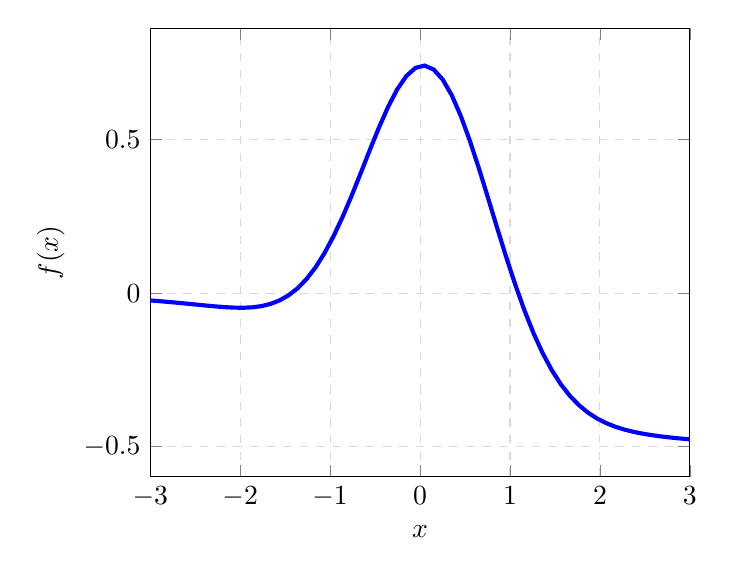
\begin{tikzpicture}
            \begin{axis}[
            grid=major, 
            grid style={dashed,gray!30},
            xlabel=$x$, % Set the labels
            ylabel=$f(x)$,
            xmin=-3,
            xmax=3]
            \addplot[mark=none,color=blue, line width=1.5pt, samples=100] {exp(-(x-0.1)^2)-0.5/(1+exp(-x))};%{exp(-x^2)-0.5*exp(-(x-2)^2)+1};
            \end{axis}
        \end{tikzpicture}
        \caption{Example of poor correspondence between local and global
        structure. If $x<0$ is initialized, gradient descent will lead us in
        negative direction of $x$. However, this leads away from the global optimum
        on the right.}
        \label{fig:Poor_correspondence}
    \end{center}
\end{figure}

Another issue may be that there even is no global minimum. This happens for
example with the usage of the softmax, where the weights are increased without
bound even when the accuracy is very good. This occurs because the actual labels
for the softmax can only approach 1 with larger values, but never actually reach
it.  On solution to the second phenomena would be label smoothing, where instead
of a hard 0-1 coding of the classification, each of the 0 are replaced by
$\frac{k}{\textrm{\# of output units }-1}$, and the label for the true
classification is replaced by $1-k$. The network is now able to
resemble the labels without extreme output values.


\subsubsection{Initialization strategies}\label{sub:Initialization_strategies}
In the last section, the poor correspondence between local and global structure
was shown. Initializations at the wrong place on the loss landscape lead to a
gradient descent in a direction away from the global optimum. But because we
don't know the shape of the loss landscape in advance, no initialization can
guarantee a good solution or even convergence at all. However, some strategies
seem to perform better than other and have become widely used.

The first and only known property of initialization is that is has to be
asymetric. This means that two units that share the same input must have
different weights attached to these inputs. If this is not the case, a
deterministic optimization algorithm will update both these parameters in the
same way. To break this symetry, the weights are initialized randomly. If a
gaussian or uniform distribution is used does not seem to matter.

However, the range of these functions is important. Wide distributions have a
stronger symetry breaking effect, but come with the risk of exploding gradients
as discussed in section \ref{sub:Vanishing_gradient}. The problem of vanishing
gradients arise if the distribution is too small. The statictical viewpoint
suggests a initialization to small weights nevertheless. Here, large weight
initialization is seen as a large gaussian prior on which and how the units
interact. As we have no reason to encourage one interaction over another, the
weights should be as small as possible. 

Some heuristics try to balance these different motivations. One of the most
famous one is the normalized initialization from Glorot
\cite{glorot2010understanding}. For a fully connected layer of $m$ inputs and
$n$ outputs, the weights should be initialized according to a uniform
distribution:

\begin{align}
    W \sim U(-\sqrt{\frac{6}{m+n}}, \sqrt{\frac{6}{m+n}})
\end{align}

The biases are normally initialized to a constant. A value of 0 seems to behave
well for most applications.




\subsubsection{Stopping criteria}\label{sub:Stopping_criteria}
In traditional optimization, simple heuristics are used to determine the point
of stopping, like a gradient of 0. However many local extrema exits on the loss
landscape of deep neural networks, making a stop at the first extremum
unattractable.

Therefore, other stopping criteria have been developed. What we normally see in
terms of performance is an initial decrease in training loss paired with an
increase in validation accuracy. But after some epochs, we enter the overfitting
region, where training loss keeps decreasing but validation accuracy also
decreases again. In early stopping, this is used the determine the stopping
point. After each epochs we store a copy of the parameter values. Then we train
the network for a fixed number of epochs. At the point when the validation error
starts to rise again, we can return to the parameter values from before. As no additional
computation time is required, this is a very efficient method from a
computational perspective, but may require some extra storage. This apporach is
very different to traditional optimization, as gradients may still be very large.



\subsection{Algorithms}
\subsubsection{Stochastic Gradient Descent}\label{SGD}
Stochastic Gradient Descent (SGD) is one of the most popular optimization
algorithm in deep learning. It is also one of the most basic ones, as it only
takes the gradient at the current position into account. In contrast to normal
gradient descent, SGD computes the gradient on minibatches, not on the whole
dataset. Nevertheless, as long as the training data is only used once, SGD gives
an unbiased estimate of the true gradient, see Section \ref{sub:Minibatch}. 

\begin{algorithm}
    \hypertarget{alg:SGD}{}
    \begin{algorithmic}[1]
        \caption{Stochastic gradient descent from \cite{Goodfellow-et-al-2016}}
        \REQUIRE learning rate $\lambda$
        \ENSURE a trained neural network
        \STATE initialize the network, dataset and training parameters
        \WHILE{stopping criteria is not met}
            \STATE sample minibatch of $m$ examples ${x^{(1)}, ... ,x^{(m)}}$
            \STATE compute gradient estimate $\hat{g}=\frac{1}{m} \nabla_\theta \sum_i L(f(x^{(i)};\theta),y^{(i)})$
            \STATE apply parameter update $\theta=\theta-\lambda\cdot\hat{g}$
        \ENDWHILE
        \STATE \textbf{return: the trained network}
    \end{algorithmic}
\end{algorithm}

First, the network is initialized. Then, the training loop repeats, until the
stopping criteria is met. At the beginning of each iteration, a minibatch is sampled. Then, the
gradients are calculated, multiplied by the learning rate $\lambda$ and finally
applied to update the parameter values.


\subsubsection{Learning rate decay}\label{sub:Learing_rate_decay}
One of the most important hyperparameters of SGD is the learning rate. While the
optimal learning rate differs for every problem, it is important to decay the
learning rate with the number of epochs. Initially, it is good to choose a large
learning rate. This leads to fast learning at the beginning, and avoids the
algorithm getting stuck in areas of high loss. As the number of epochs
increases, it is important to shrink the learning rate. Since SGD is a
stochastic algorithm, its gradient is inaccurate. Even when we find a local
minimum with a gradient of 0 on the minibatch, the true gradient will not be 0.
A small learning rate secures to get close to the minimum while not overshooting
it repeatedly.

How the learning rate is decayed varies from algorithm. A popular decay is
piecewise constant decay, where the learning rate is decayed by a constant
factor $\gamma$ after a fixed number of epochs.
\begin{align}
    lr = lr_0 \cdot \gamma^{\lfloor epoch/stepsize \rfloor}
\end{align}
Another popular algorithm is cosine decay, where the learning rate is decayed
continously.
\begin{align}\label{eq:cosine_decay}
    lr_t = lr_{min} + \frac{1}{2} (lr_{max} - lr_{min})(1+cos(\frac{T_{cur}}{T_0}\pi))
\end{align}
Here $lr_{min}$ and $lr_{max}$ define the range of the lr, $T_{cur}$
is the current and $T_0$ is the maximum number of epochs. The advantage of
cosine decay is that the learning rate is decayed down to 0 in the defined
interval, independent of the initial learning rate. In contrast, the smallest
learning rate of step decay is dependent of the initial one.

\subsubsection{SGD with Momentum}\label{sub:Momentum}
Momentum is a popular variation of SGD. It is used to speed up the training of
SGD. The term Momentum is used, as the underlying idea is the similar to the
physical context. Consider a frictionless ball rolling down a hill. The ball
builds up speed the further it rolls down by adding the acceleration of current
gradient to the velocity. The ball will speed up, until it faces an uphill,
where it will slow down again.

In context of deep learning, we use the velocity $v$ rather than only the
current gradient $g$ to update the parameters.

\begin{align}
    v_{t+1}=m \cdot v_t - \lambda g
\end{align}
Here, $m$ controls how strong the past gradient is taken into account, while
$\lambda$ denotes the current learning rate. For the ball to build up velocity,
it requires a constant downhill motion. The same is true for this case. The
gradient can only build up, if it points in the same direction for some
consecutive updates similar to the ball. Therefore, momentum speeds up the
gradients of parameters, whose gradient is constant in one direction over
multiple epochs. Parameters with alternating gradients for example will only
experience small updates, because the different orientations of their gradient
will level out. Formally, if parameter $p$ experiences the same gradient $g$
every time, it will reach a terminal velocity of
\begin{align}
    \frac{\lambda \lVert g \rVert}{1-m}
\end{align}
This also shows that $m$ can be used to control the speed up of the
training. If $\lambda$ is kept constant, the larger $m$, the faster
training will become, as long as the gradient is constant for multiple update
iterations. A value of $m=0.9$ for example would lead to a speed up factor of
$10$, while $m=0.8$ would lead to a speed up of $5$.

\begin{algorithm}
    \hypertarget{alg:SGD_Momentum}{}
    \begin{algorithmic}[1]
        \caption{Stochastic gradient descent with Momentum from \cite{qian1999momentum}}
        \REQUIRE learning rate $\lambda$
        \REQUIRE momentum parameter $m$
        \ENSURE a trained neural network
        \STATE initialize the network, dataset and training parameters
        \WHILE{stopping criteria is not met}
            \STATE sample minibatch of $m$ examples ${x^{(1)}, ... ,x^{(n)}}$
            \STATE compute gradient estimate $\hat{g}=\frac{1}{m} \nabla_\theta \sum_i L(f(x^{(i);\theta}),y^{(i)})$
            \STATE compute velocity update $v=m \cdot v - \lambda \hat{g}$
            \STATE apply parameter update $\theta=\theta-v$
        \ENDWHILE
        \STATE \textbf{return: the trained network}
    \end{algorithmic}
\end{algorithm}

In pseudo code, SGD with Momentum in ALgorithm \hyperlink{alg:SGD_Momentum}{2}
looks similar to normal SGD in ALgorithm \hyperlink{alg:SGD_Momentum}{1}. The
only difference is line 5 and 6, where the velocity is updated and then used to
update the parameters rather than the gradient itself.

\begin{comment}
Momentum also adds a regularization effect, because it is attracted to stable
or flat minima. If the minima is too small, it won't be able to stop the
momentum and therefore the SGD will move on. That's similar to a ball, which
won't stay in a small hole but keep on going, if it's speed is larger enough.
\end{comment}





\section{Related work}

The last sections focused on general challenges of neural network optimization
and how to overcome them. This section gets into more detail on some of these
and shows current techniques in neural network optimization, some of which are the basis
for the methods and results in the following chapters.




\subsection{Wide minima and Generalization}\label{sub:Generalization}
In section \ref{sub:1}, we saw how learning differs from normal optimization,
namely that we only have acces to the training set and thus have to optimize
indirectly. With an increasing number of training epochs, the network starts to
memorize the training data. Because the data distribution of the training data
is not identical to the distribution of test data, this usually leads to a
better performance of the network on the training set than on the test set. The
difference between those performances is known as Generalization Gap. 

Strategies that are developed to deal with this problem are subsumed under the
term \textbf{Regularization}. One common reguralizer is the $L_2$ Reguralizer.
Its goal is, to encourage the weights to stay small. Small weights have some
advantages for the generalization capabilities. First of all, small weights
remove the dependency of a unit to one of its inputs. Because the weights are
really small, a strong activation cannot be solely achieved by the presence of
one input, but rather has to rely on multiple units. Therefore small changes in
the input will only cause small changes in the output, instead of the absence of
one feature for example leading to a different output. This benefits the
generalization, as the distribution of training and test data is slightly
different. Formally this can be incorporated in the loss function by adding the
squared $L_2$ norm:
\begin{align}
    L= L(f(x;\theta), y)+l \cdot \lVert \theta \rVert_2^2
\end{align}
The paramter $l$ controls the strength of the $L_2$ and has to be adjusted individually
for each problem.

Other work has gone into understanding the connection to the loss surface.
Hochreiter \& Schmidhuber \cite{hochreiter1997flat} argued that flat minima
have better generalization capabilities. A flat minima is a region where the
loss stays constant in contrast to sharp one, where small steps can increase
the loss significantly. Therefore, flat minima will perform constantly even for
small changes in the input, whereas sharp minimas will lead to an increase in
generalization error. Support also comes from the minimum description length
theory, which states that fewer bits are needed to describe a flat minimum than
a sharp. Lower complexity leads to a better generalization error. The idea is,
that in the network we try to compress the data. The more we compress the data
while also beeing able to resemble it, the more of the structure of the data we
uncover. Therefore, a model with lower complexity can fit the underlying data
better and achieve a better generalization error. Keskar et al.
\cite{keskar2016large} draw the same conclusion. They also provide a solution
for finding flat minima in using small batch sizes, see chapter
\ref{sub:Minibatch}.

Work from Dinh et al. \cite{dinh2017sharp} however contradicts this view. They
argue that the notion of flat is problematic in the context of deep learning, as
the loss surface is very complex. Based on previous definitions from the
papers above, they construct parameter values which lie on a sharp point of the
surface, but are also able to generalize well. Therefore, at least some caution
is needed when arguing about flatness beeing a reason for generalization
capabilities.

\subsection{Loss landscape}\label{loss_landscape}
Section \ref{prob:5} showed that the poor correspondence between local
and global structure may propose a major issue for optimization. Bad
initializations may lead to path which moves away from the global otimum, often
without chance to recover. Initialization strategies try to adress this problem,
but cannot guarantee to solve it.

An open question is if this suboptimal structure is present in deep neural
networks. Fengxiang et al. \cite{he2020piecewise} showed that there exist
infinitly many local minima which are of higher cost than the global one.
Furthermore, these minima are arranged in enclosed areas, where each minima
within one area has the same loss as the others and is also connected to them by
paths of low loss. These areas are seperated from each other by
nondifferentiable boundaries. Unfortunally, it remains unclear if different areas 
are of different cost. If this is the case, this would propose a major problem.
When the training process gets into one of these areas, it is likely to get
stuck, probably in an area of suboptimal cost. A trivial way to recover is not
present at the moment.

Draxler et al. \cite{draxler2018essentially} get to a smiliar result, that local
minimas are connected by paths of low loss. On these paths, the training loss stays the
same to the one of the connected minima, while the test error rate slighly
increases.

Fort \& Jastrzebski \cite{fort2019large} put this in a more formal context. For
each tuple of dimensions, they construct disks to describe the hyperplanes
defined by them. They calls these hyperplanes wedges. One property is that the
paths of low loss described above lay on these wedges. Therefore the
connecting path for two points on different wedges has to pass through the
intersection of them, and their direct connection is an area of high loss.
When viewed from an cross-section, these paths from a tunnel. Some techniques
to improve optimization have similar effects on the size of these tunnels,
namely they widen them. This happens for example for higher $L_2$ regularization
\ref{sub:Generalization}, smaller batch sizes \ref{sub:Minibatch} or higher
learning rates.


\subsection{Cosine Decay with Warm Restart}\label{sub:cosine_decay}

In section \ref{SGD}, learning rate schedulers were introduced. The idea was to
have a high learning rate at the beginning for fast improvements, and then a
decrease to fine adjust the parameters. One scheduler was cosine decay, with the
formula \ref{eq:cosine_decay}. In the paper of Loshchilov \& Hutter
\cite{loshchilov2016sgdr}, they use this scheduler in combination with another
technique, called warm restart. In constrast to the naive approach, where the
learning rate is only decayed once, warm restart decayes until a fixed number of
epochs, and then set back up to the inital learning rate. This procedure can be
repeated for several times. The idea is, that a high learning rate leads to
exploration of the loss landscape, while a low learning rate leads to
exploitation.

In their results, at every restart, the performance becomes worse for some
epochs due to the high learning rate. But when the learning rate decays again, the
previous performance is reached and even topped. this leads to a new state of
the art result at 3.14\% test error for Wide-Residual-Net 28-20 on CIFAR-10.
Their method also perfoms better when compared to step decay. 


\subsection{Ensemble methods}\label{sub:Ensemble_Methods}
The general idea of ensemble methods is to combine the predictions of multiple
models to get a more accurate prediction. The fact that this leads to an
improvement can be seen in a simple regression problem. Suppose there exist $k$
models that make a prediction error of $e_i$ with mean 0, variance $E[e_i^2]=v$ and
covariances $E[e_i e_j]=c$ on every particular prediction. If these models are
combined, the variance reduces to 
\begin{align}
    E[(\frac{1}{k} \sum_i e_i)^2]=\frac{1}{k^2}E[\sum_i (e_i^2 + \sum_{j\neq i} e_i e_j)]=\frac{1}{k}v+\frac{k-1}{k}c
\end{align}
If all models make the same predictions, so $c=v$ for all combinations of
models, then the sum decomposes to $v$, so the prediction error is the same as
before. On the other hand, if $c=0$, the prediction error is reduced by a factor
of $\frac{1}{k}$. Therefore, for ensemble methods to be succesfull, every individual model
has to achieve a low prediction error, while the predictions of all models
should be as different as possible. While the low error is achieved in deep
learning by standard training of the models, there are several approaches to
ensure that the correlation between the models stays los.

The first idea would be to vary the training data for the model. One way this
can be realized is by k-fold cross-validation. Here, we split the training data
into $k$ different smaller datasets. Then we train $k$ independent networks on one
of these subsets. This however decreases the size of the training set for each
model drastically. Therefore another common approach is bagging
\cite{breiman1996bagging}, where we draw a subset from the training data, but
with replacement. Here, individual examples might occur in more than one
training set. Training on different datasets leads to lower correlation, which we
can use to our advantage as we have seen above. As the number of training
examples is limited however, we might not be able to sustain a sufficient low
error.

To use the whole training data while also creating different models, we can
alternatively alter the model itself. An naive approach would be to just use
different model architectures. If we want to use the same architecture for all
models, we can vary the parameter initilializations. This is often enough to
create models that have different predictions. However, for every initialization
a network has to be trained from beginning, which can become very costly. A
novel approach is to train one network, but to take snapshots of the network
parameters at different steps. This approach adds no additional cost, as we only
train one network. To ensure different networks, Huang et al.
\cite{huang2017snapshot} use the method of cosine decay with warm restarts
\cite{loshchilov2016sgdr}, as explained in section \ref{sub:cosine_decay}.
Recall that at each restart, the learning rate is set up to the initial learning
rate. This results in the optimizer taking larger update steps and consequently,
the network parameter values will distance from their current state. The
snapshots of the networks are taken before each restart, as the network
converges to area of low loss when the learning rate is low. With this method,
we are able to get models with low correlation, low error and no additional cost.

After we have ensured that the conditions for the models are met, we have to
think about how to combine threi predictions. For the case of classification
with the use of softmax layer, we can use a technique called model averaging.
Here, we sum the predictions of the individual models, and take the class with
the highest prediction, as in standard classification. Formally, if the
probability output of a model i for a given class c is $p_{c_i}$, then we sum
the probabilites of each individual model: $p_c = \sum_i p_{c_i}$. To predict
the class we take $argmax_c(p_c)$. If we have reasons to believe in a better
prediction of one model over another, we can add weights $w_i$ to the
probabilites of the individual models: $p_c = \sum_i w_i \cdot p_{c_i}$.


\begin{comment}
Further aspects that could be included:
- classififcation in general
- cross entropy loss and loss functions
- gradient descent
\end{comment}